\documentclass[aspectratio=169]{beamer}
\usetheme{default}
\beamertemplatenavigationsymbolsempty
\setbeamertemplate{itemize items}[circle]
\usepackage{booktabs}
\usepackage{graphicx}

\title{PPL Benchmark --- Update}
\author{}
\date{}

\begin{document}

\begin{frame}{Probabilistic-programming benchmark}

  \begin{minipage}{0.84\textwidth}
  \begin{itemize}
    \item \textbf{What.} Language-neutral PP problems. LLM writes the program;
          graded by whether its \emph{answer / posterior} matches verified
          ground truth --- not text match. Across WebPPL, Pyro, Stan.

    \medskip
    \item \textbf{Why multi-language.} PPL is low-resource --- few
          (problem, solution) pairs. A multilingual collection lets us
          translate across languages, multiplying the usable corpus from the
          same problems.

    \medskip
    \item \textbf{The hard part.} Needs verified ground truth per language
          \emph{and} one comparator that judges distributions, not strings.

    \medskip
    \item \textbf{Latest.} Ran 7 models $\times$ 3 languages (see next slide).
          A large share of failures trace to the \emph{prompt}, not the model
          --- tightening the prompt contract lifts scores substantially.
  \end{itemize}
  \end{minipage}%
  \hfill
  \begin{minipage}{0.14\textwidth}
    \raggedleft
    
\includegraphics[width=18mm]{qr.png}
  \end{minipage}

  \vfill
  \footnotesize Live demo $\to$ \texttt{pplgym.kingdomofends.org}

\end{frame}

\begin{frame}{Results --- pass rate, 7 models $\times$ 3 languages}

  \begin{center}
    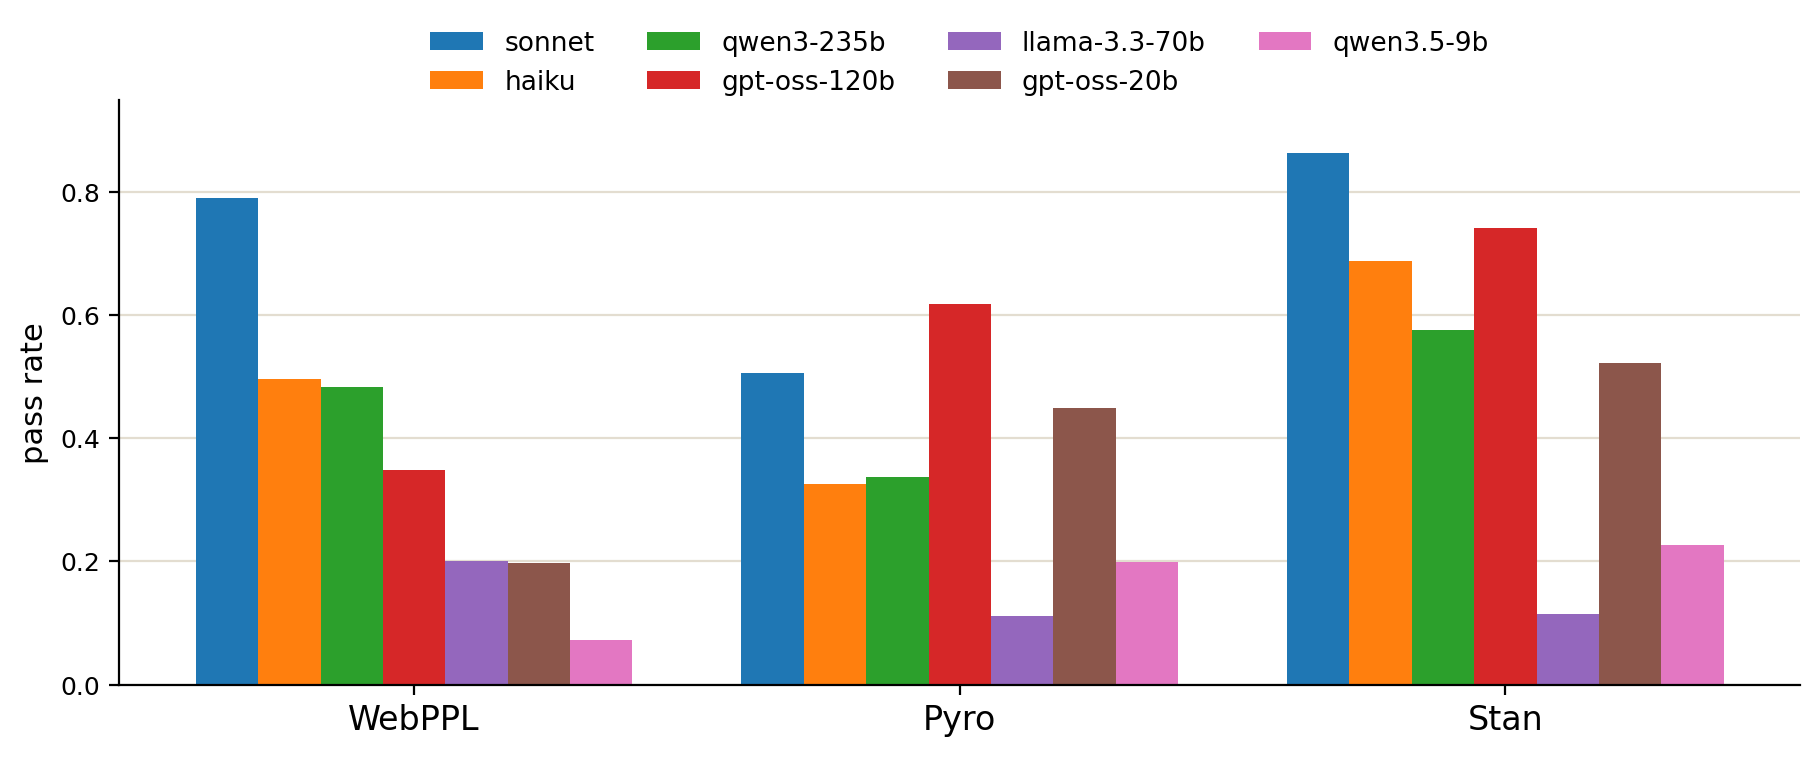
\includegraphics[width=0.95\textwidth]{results.png}
  \end{center}

  \vspace{1mm}
  \footnotesize Fraction of problems whose answer lands inside the measured
  tolerance band.

\end{frame}

\end{document}
